\documentclass[12pt,letterpaper,english,bibliography=totocnumbered, abstract=on]{scrartcl}

\usepackage{indentfirst}
\usepackage[titletoc]{appendix}
\usepackage[T1]{fontenc}
\usepackage[latin9]{inputenc}
\usepackage{color}
\usepackage{babel}
\usepackage{verbatim}
\usepackage[unicode=true,pdfusetitle,
bookmarks=true,bookmarksnumbered=false,bookmarksopen=false,
breaklinks=true,pdfborder={0 0 0},pdfborderstyle={},backref=false,colorlinks=true]
{hyperref}
\hypersetup{linkcolor=blue,citecolor=blue,urlcolor=blue}

\usepackage{booktabs}
\usepackage{multirow}
\usepackage{adjustbox}
\usepackage{threeparttable}
\usepackage[table]{xcolor}
\usepackage{csquotes}
\usepackage{soul} % for hiliting text: \hl

\usepackage[backend=biber, style=authoryear, maxbibnames=99, dashed=false]{biblatex}
\setlength\bibitemsep{2\itemsep}
\addbibresource{CRB.bib}

\usepackage{pdfpages}
\usepackage{float} % Allows use of H to place floats

\usepackage{pgfgantt}

\usepackage{framed}

\usepackage{datetime2}

% Prevent page breaks within paragraphs
% https://tex.stackexchange.com/questions/21983/how-to-avoid-page-breaks-inside-paragraphs
\widowpenalties 1 10000

\begin{document}

%\titlehead{Titlehead}

\title{Roadside Video Surveys of Coconut Rhinoceros Beetle Damage}

\author{Aubrey Moore}

\date{\DTMnow}


\maketitle

\tableofcontents

\footnote{The most recent version of this document can be downloaded from\\
\url{https://github.com/aubreymoore/CRB-trap-improvement/blob/master/results.pdf}.}

\pagebreak

\section{Background}

\cite{vaqalo_coconut_2017}

\section{Data Acquisition}

\subsection{Mounting a Smart Phone on a Vehicle}

Preliminary work show that mounting the smart phone externally produces much better results than mounting the phone internally as a dash cam. This eliminates problems cause by dirty windshields and internal reflections.  

A smart phone can be mounted externally using a ball and socket anchored using a magnet (\ref{fig:mount}).

Optimal placement of the smart phone camera appears to be above the right-hand corner of the windshield (passenger side in the US) 


\begin{figure}[h]
	\centering
	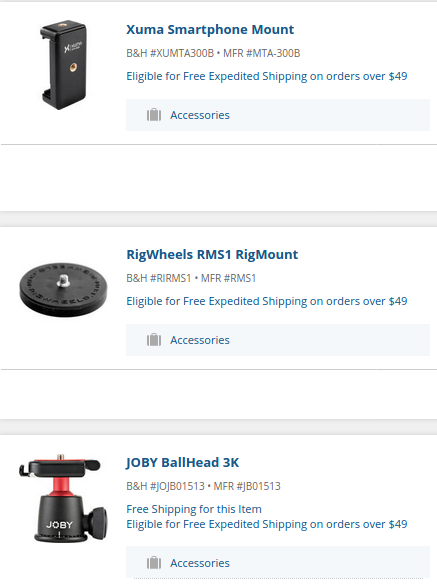
\includegraphics[width=0.7\linewidth]{images/mount}
	\caption{Smart phone mount.}
	\label{fig:mount}
\end{figure}

\subsubsection{Setting the Direction of View Angle}

The direction of view angle has two components, a horizontal angle with respect to direction of travel and a vertical angle. The horizontal angle is set using the scale at the base of the ball joint. The vertical angle is set using a free Android app called Clinometer (\url{https://play.google.com/store/apps/details?id=net.androgames.clinometer}) (Fig. \ref{fig:clinometer}).  

Optimal angles for direction of view appear to be 45 degrees to the right of direction off travel and 15 degrees above horizontal.

\begin{figure}[h]
	\centering
	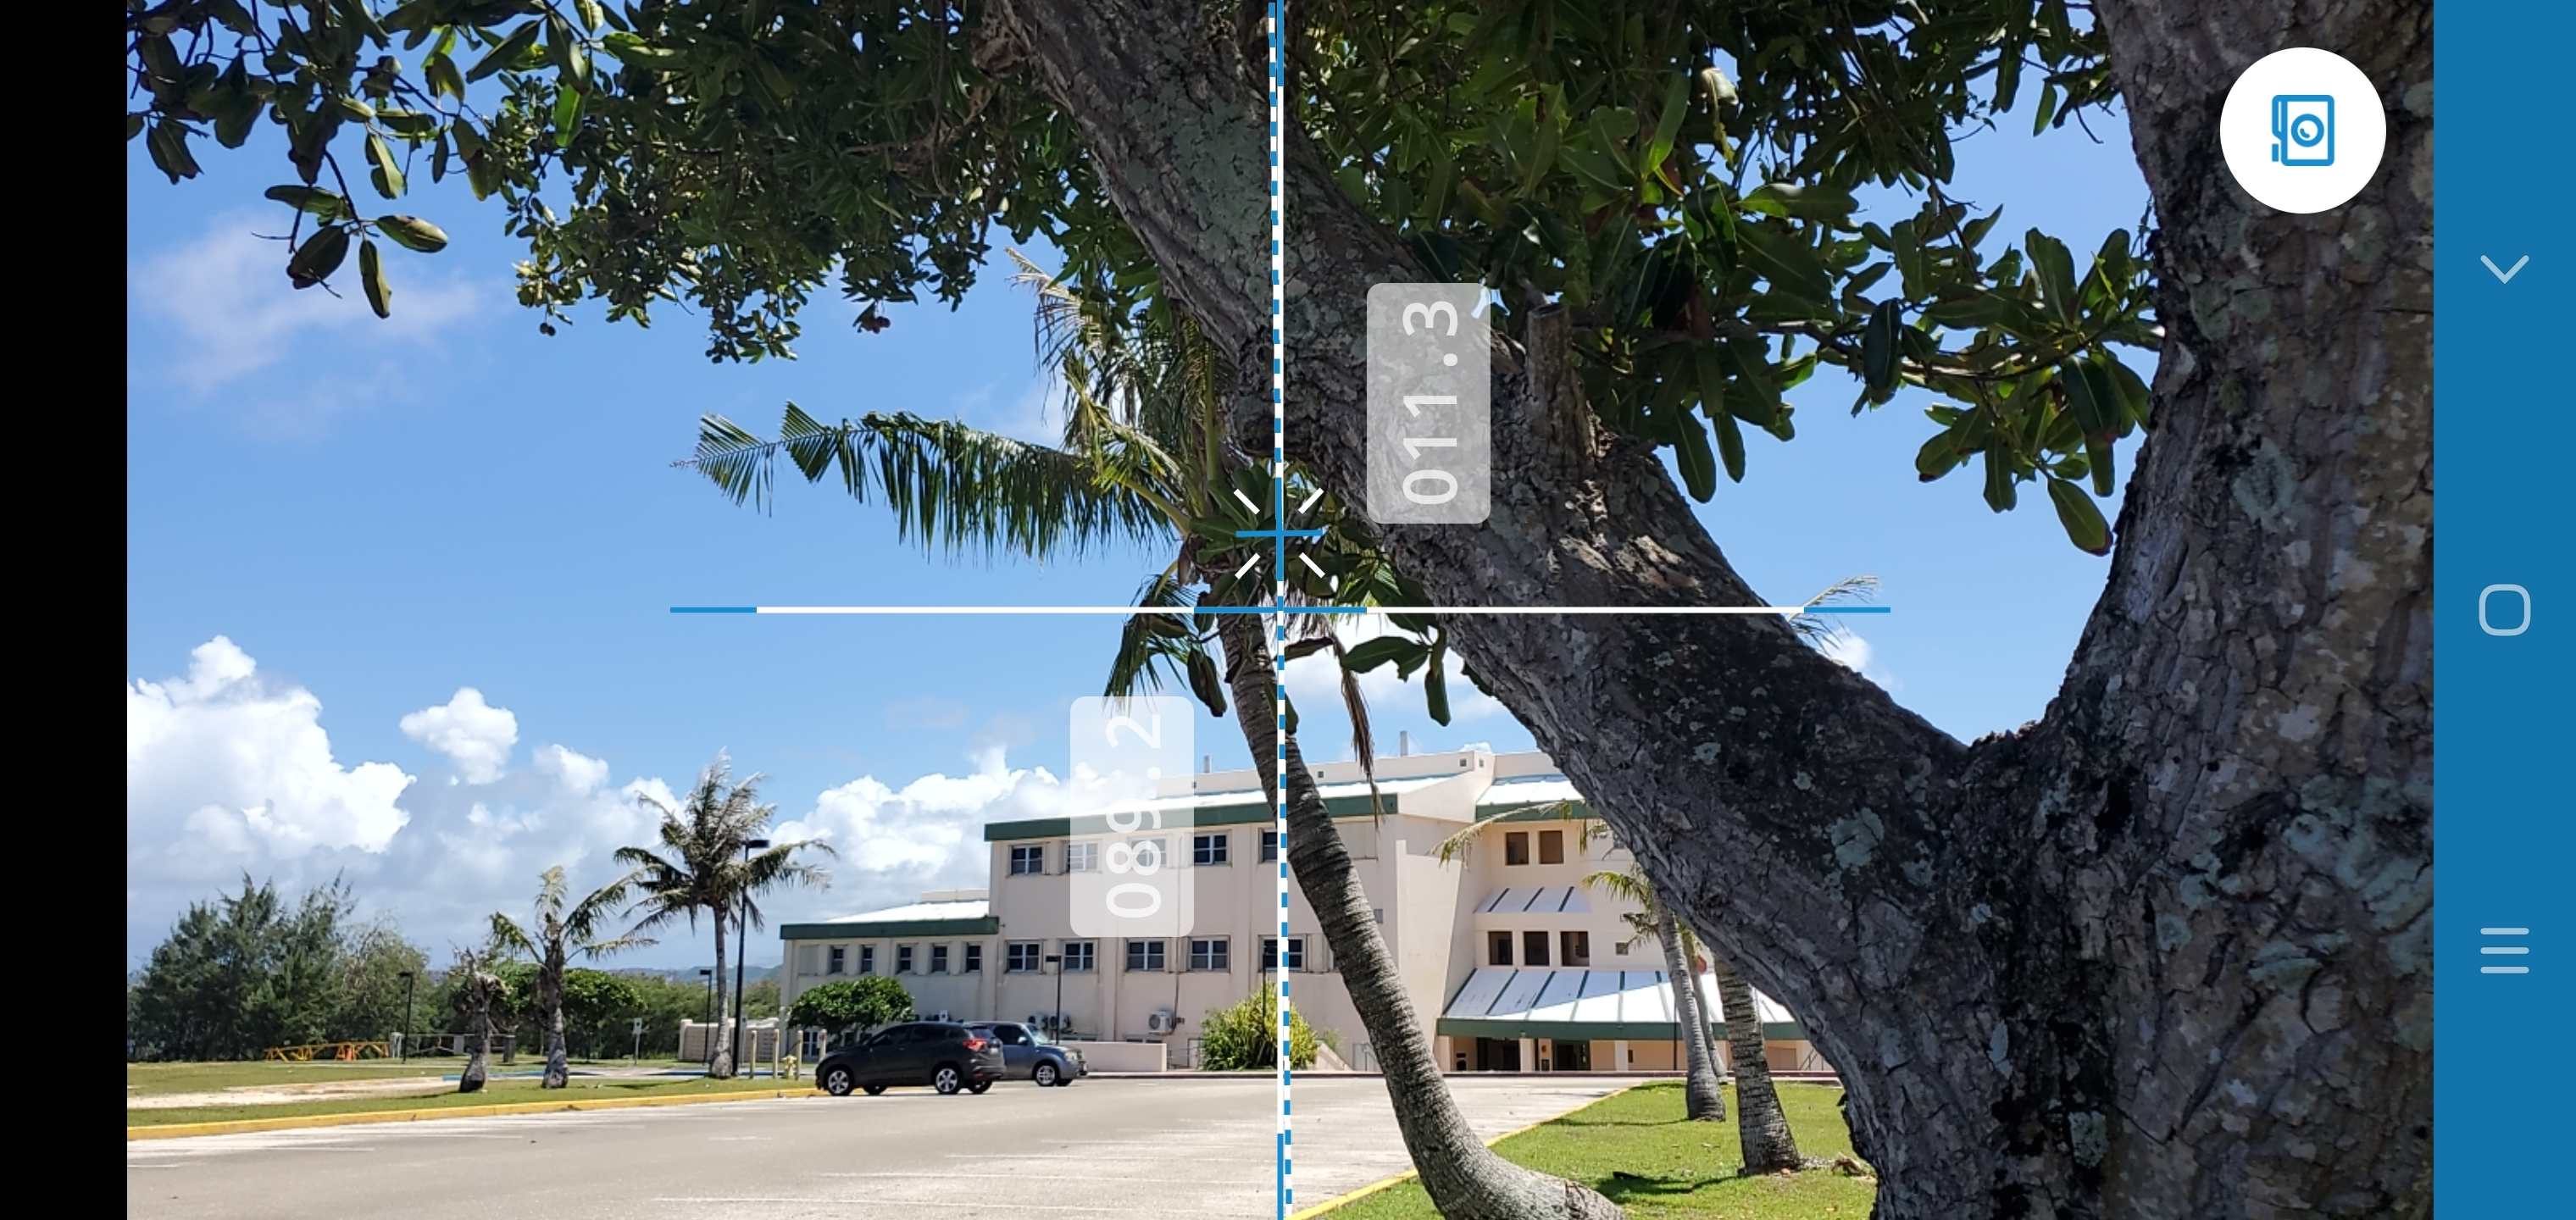
\includegraphics[width=0.7\linewidth]{images/clinometer}
	\caption{Setting camera angles using Clinometer app.}
	\label{fig:clinometer}
\end{figure}


\subsection{Parameter Choices}

\subsubsection{Camera and Lens}

We are currently using a Samsung Galaxy S10 Smart Phone.  This phone is equipped with a 16MP ultra-wide-angle camera for 123\textdegree{} field of view which seems to be a good  choice for this application.

\subsubsection{Resolution}

Maximum resolution for videos recorded with the ultrawide angle camera is 4K 3840x2160 (16:9, 8.29MP). Initial recordings were made using this resolution, but this can probably be reduced without significant loss of precision.

\subsubsection{Frames per Second}

Standard frame rate is 30 fps. Initial recordings were made using this rate, but this can probably be reduced without significant loss of precision.

\subsection{Using the Open Camera App}

Open Camera (\url{https://opencamera.org.uk/}) is a FOSS app for Android smart phones which enables much better control of hardware features than the default Camera app provided with Samsung phones. 

Open Camera offers a plethora of settings which can be saved in a configuration file for later use. 
For screenshots of \textit{Video settings} see figures \ref{fig:videosettings1}, \ref{fig:videosettings2}, and \ref{fig:videosettings3}. 


\begin{figure}[h]
\centering
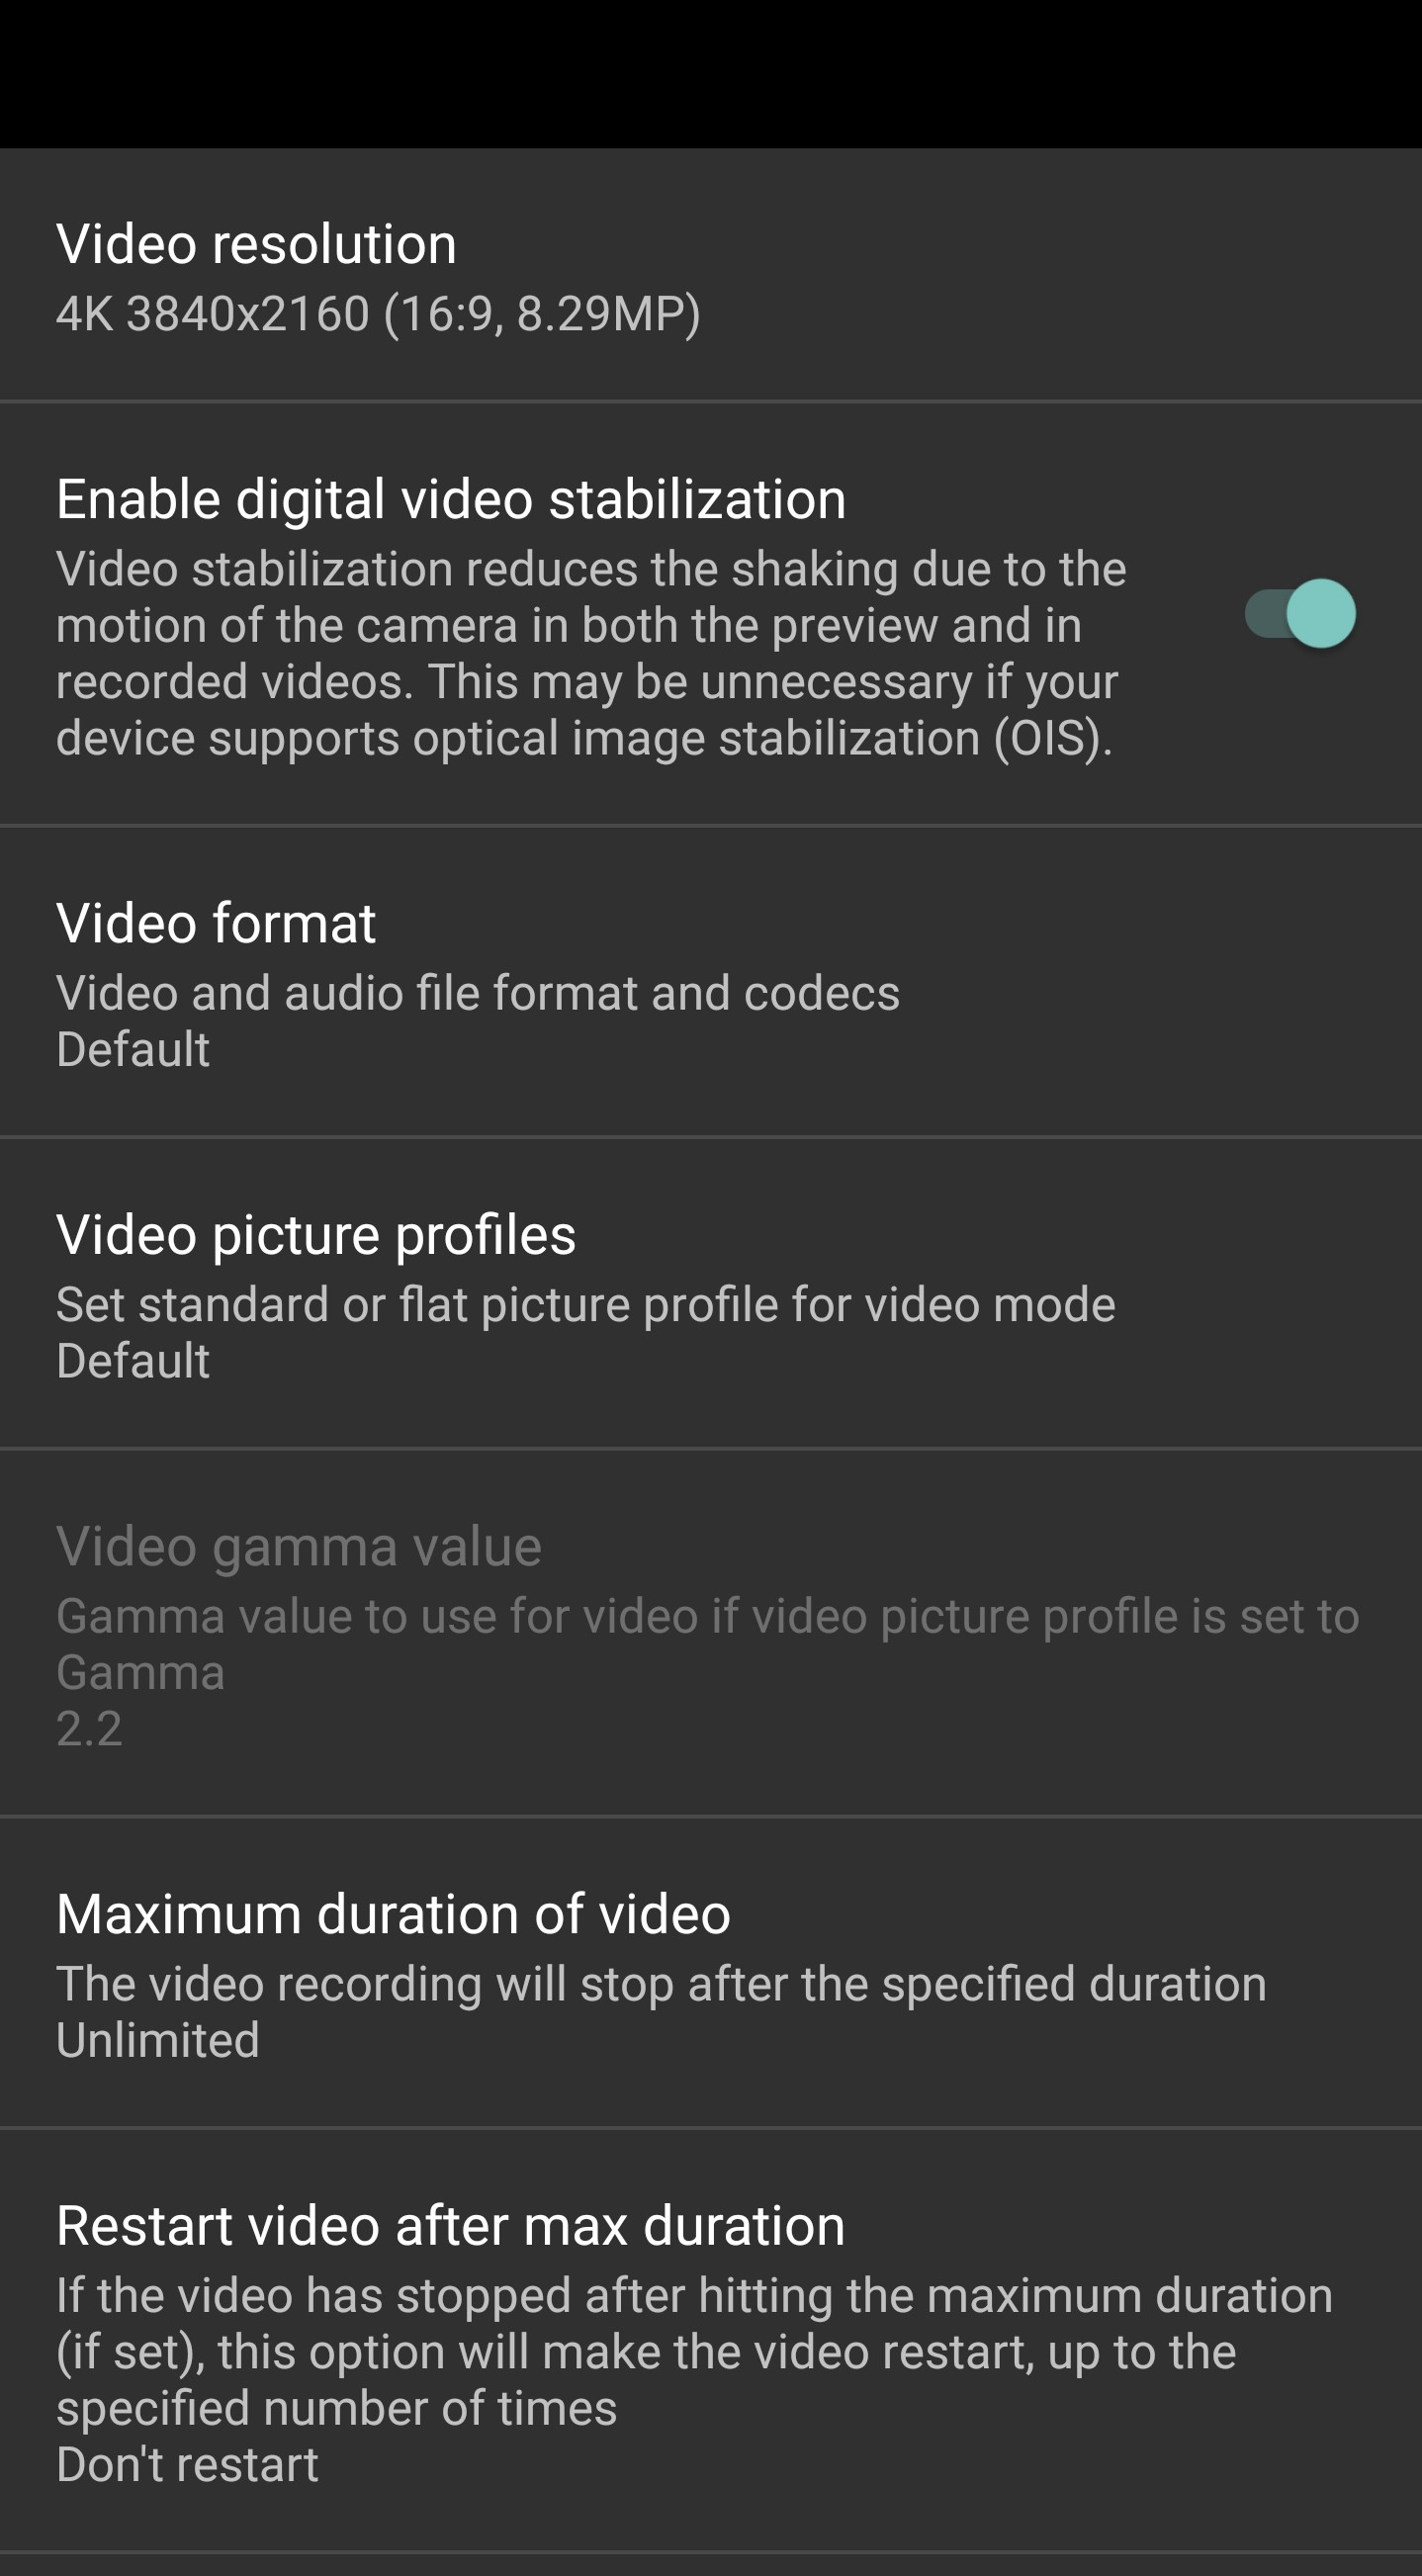
\includegraphics[width=0.7\linewidth]{images/videosettings1}
\caption{Video settings (1/3).}
\label{fig:videosettings1}
\end{figure}

\begin{figure}[h]
	\centering
	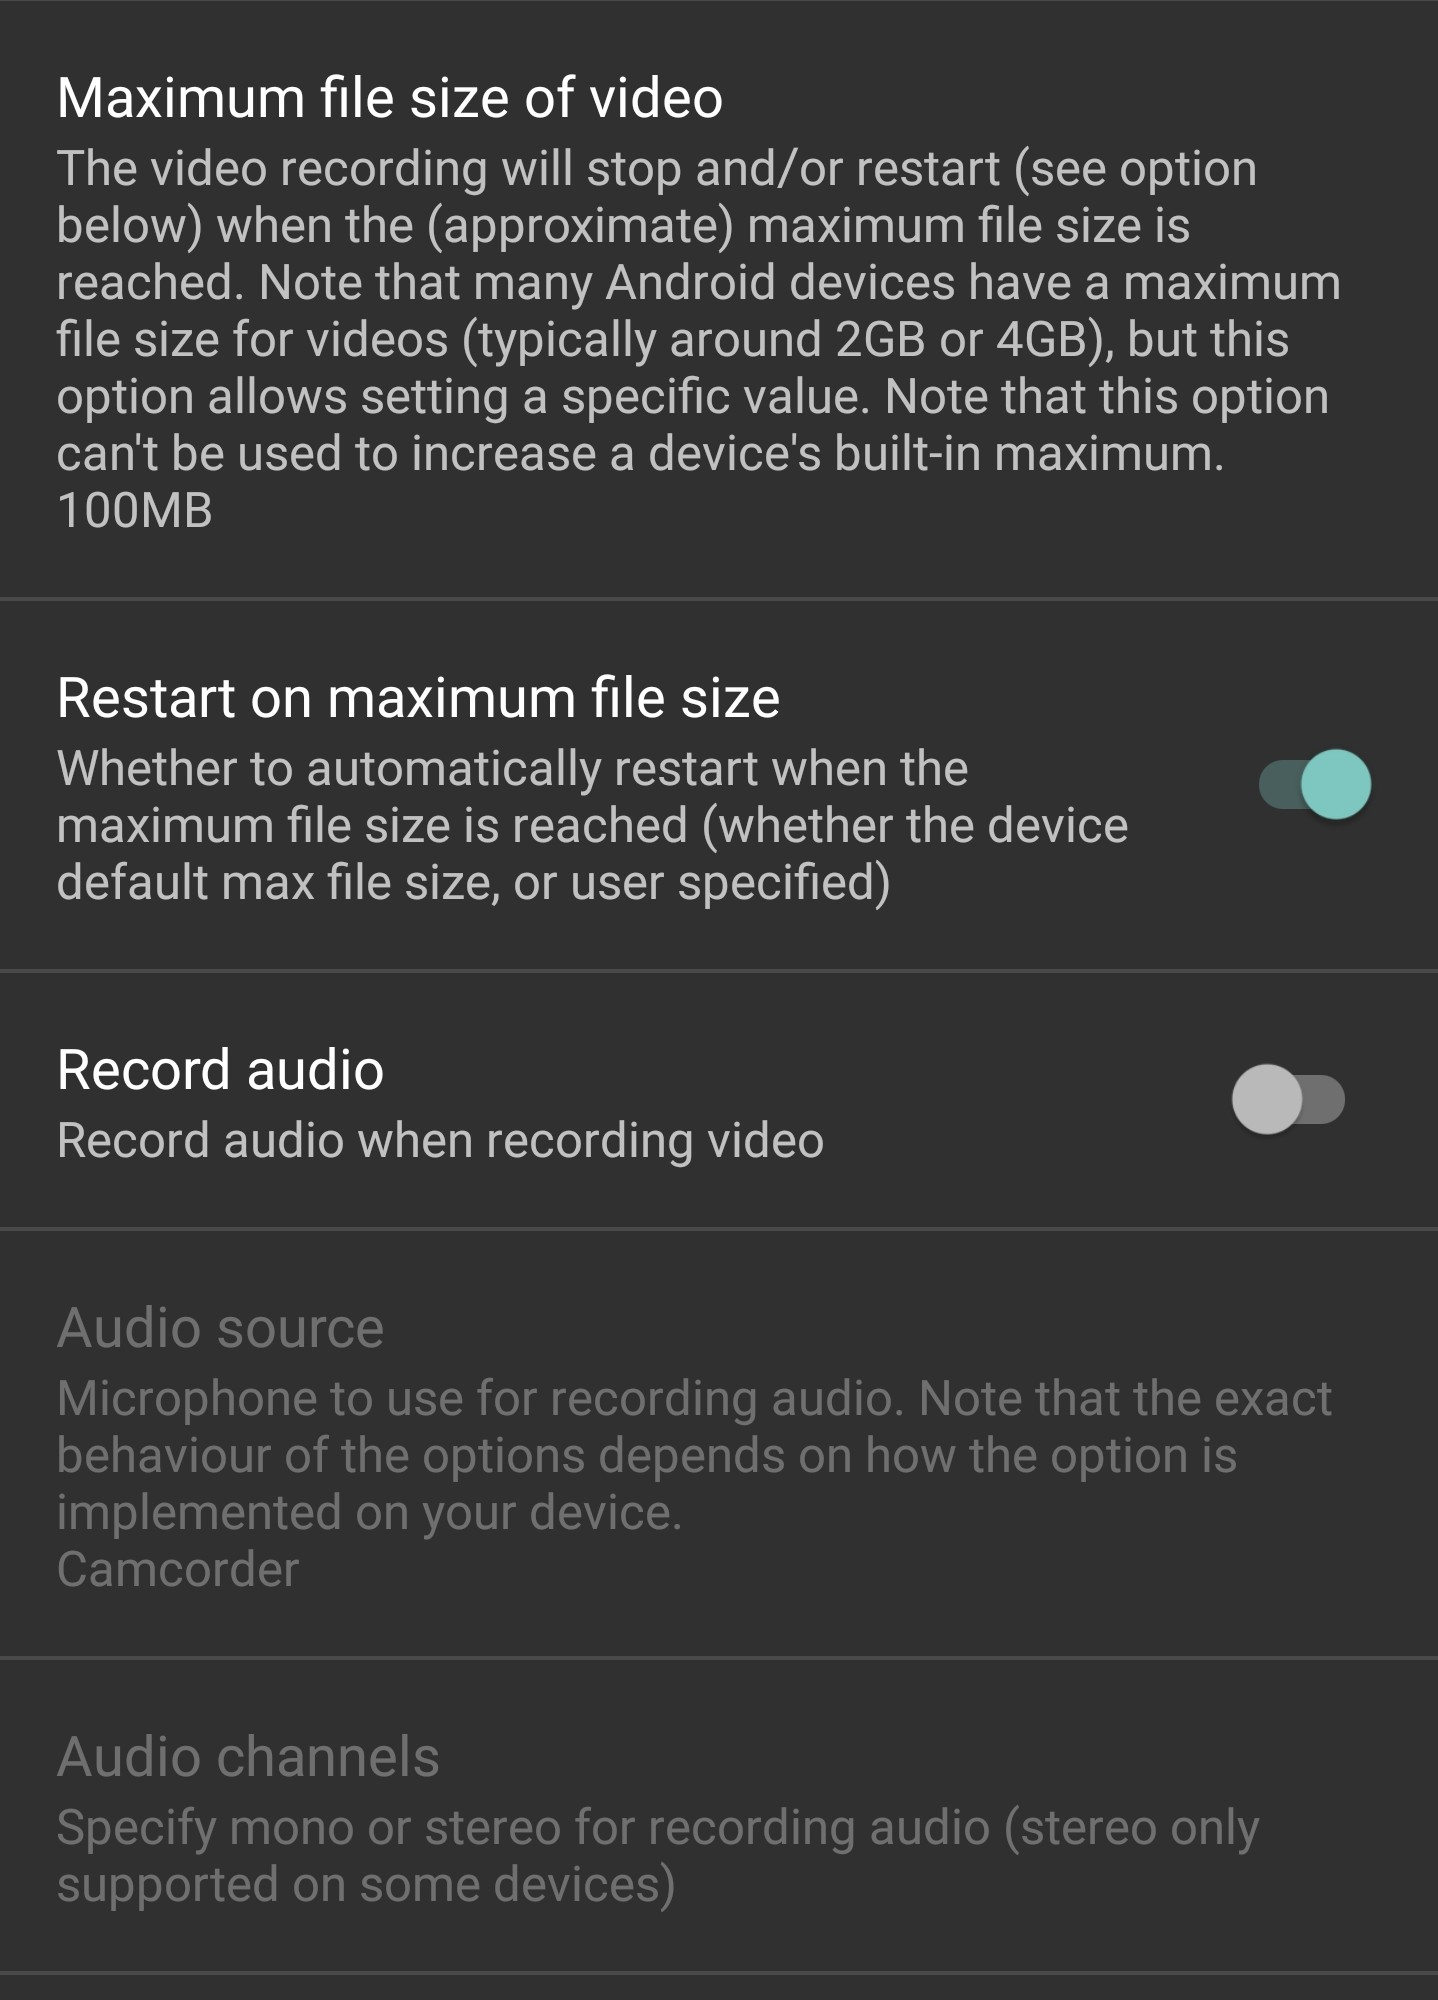
\includegraphics[width=0.7\linewidth]{images/videosettings2}
	\caption{Video settings (2/3).}
	\label{fig:videosettings2}
\end{figure}

\begin{figure}[h]
	\centering
	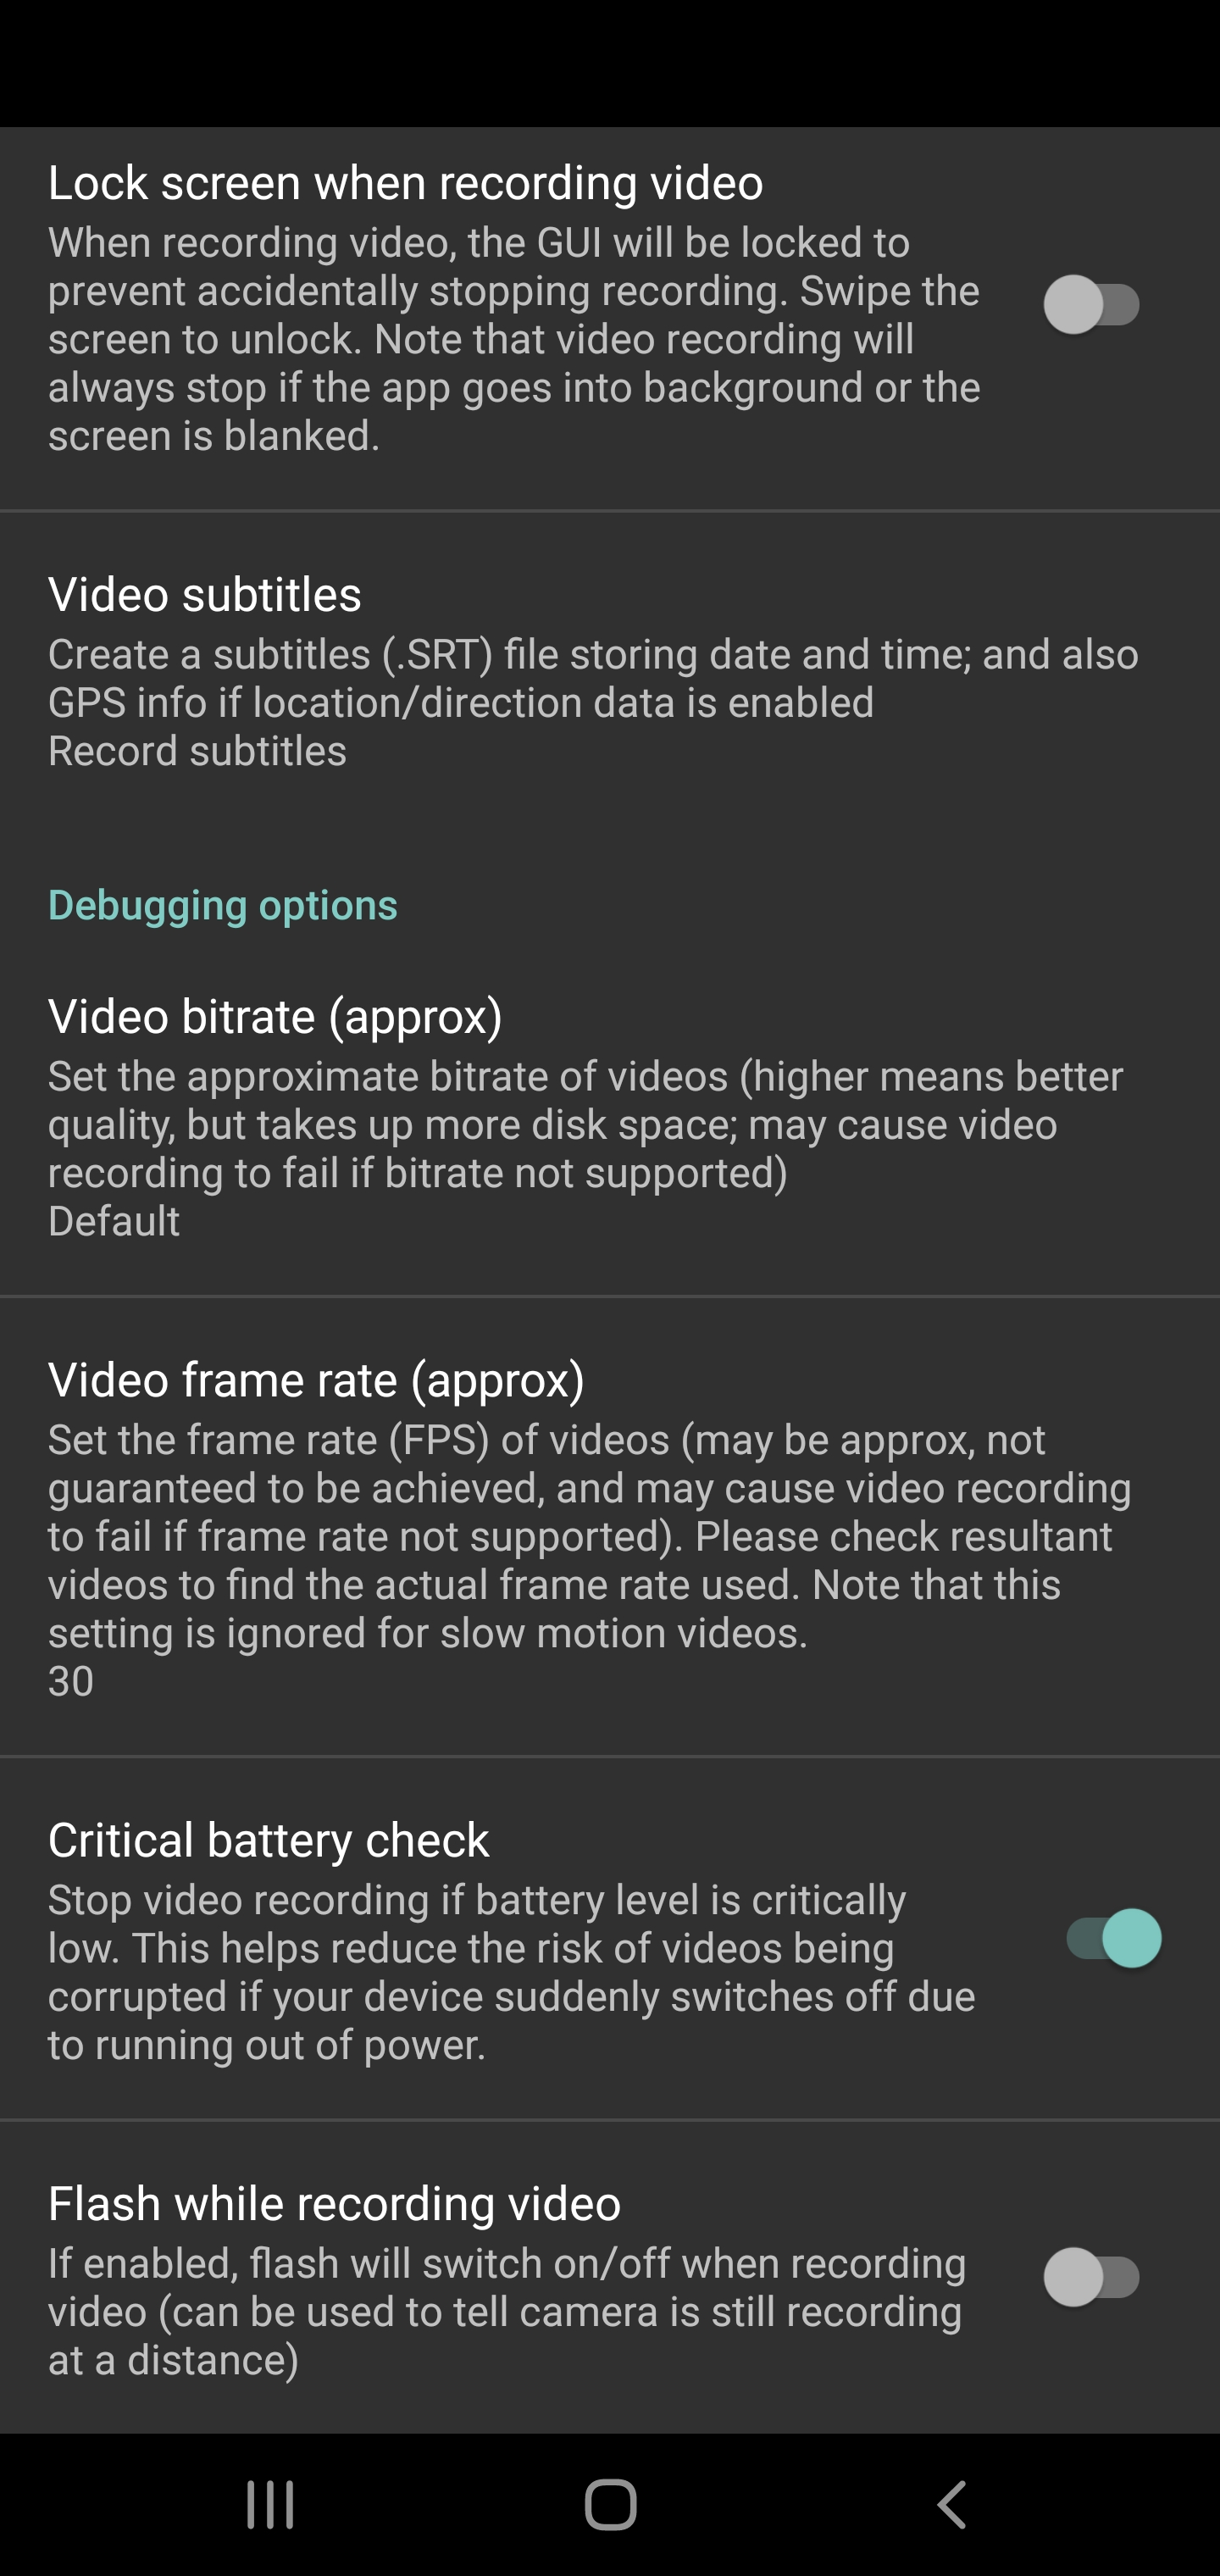
\includegraphics[width=0.7\linewidth]{images/videosettings3}
	\caption{Video settings (3/3).}
	\label{fig:videosettings3}
\end{figure}

\subsection{Georeferencing}

Although Open Camera has an option to georeference video frames, this feature proved unreliable in preliminary tests. As an alternative, it was decided to use a free called GPSLogger which logs timestamped GPS coordinates to a file at a frequency of once per second.

The author has cobbled together a jupyter notebook called georef which uses the GPSLogger log to calculate the GPS coordinates for each frame in a video recording. 

\printbibliography	

\end{document}
